%-----------------------------------------------------------------
% TITLE PAGE
%-----------------------------------------------------------------
	% deactivate header and footer
	\pagestyle{superempty}
	\newlength{\centeroffset}
	\setlength\centeroffset{(\chevin-\outmar-0.5cm)/2}

	\begin{tikzpicture}[overlay, remember picture]
	\node[
	]() at ([xshift=\centeroffset,yshift=8.5cm]current page.center) {
		\Huge \titlefont\textbf{Pocket Checklist}
	};
	\node[
	]() at ([xshift=\centeroffset,yshift=7cm]current page.center) {
		\resizebox{10cm}{!}{\titlefont\textbf{\colorbox{color1}{\textcolor{white}{\aircraftlong}}}}
	};
	\node[
	]() at ([xshift=\centeroffset,yshift=5.5cm]current page.center) {
		\Large \titlefont\textbf{\colorbox{color1}{\textcolor{white}{REV: \today}}} \blue{}
	};
	\node[
	]() at ([xshift=\centeroffset,yshift=-1cm]current page.center) {
		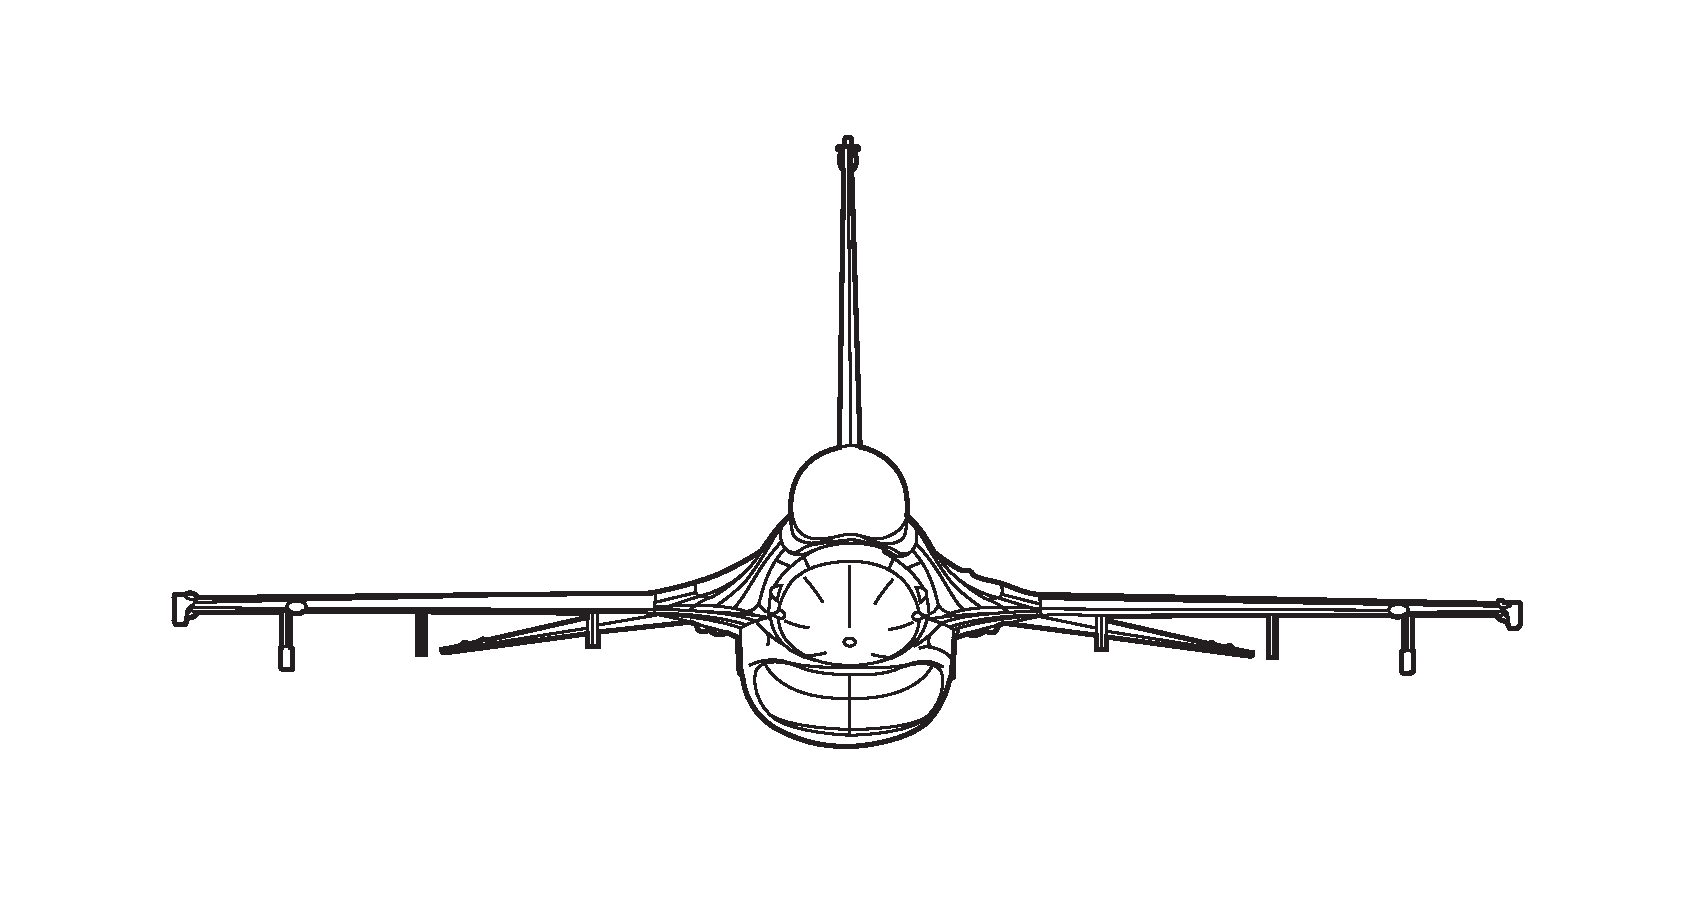
\includegraphics[
			width=0.95\linewidth
		]{F16_Front.pdf}
	};
	% Black area for white chevrons
	\fill[color1]
		([xshift=\outmar, yshift=0.2cm]current page text area.north east) --
		([xshift=\outmar, yshift=-\botmar]current page text area.south east) --
		([xshift=\chevin-0.5cm, yshift=-\botmar]current page text area.south east) --
		([xshift=\chevin-0.5cm, yshift=0.2cm]current page text area.north east) --
		cycle;
	\end{tikzpicture}
	
	% label for hyperrefs back to frontpage
	\label{frontpage}
	% make chevrons
	\thumbfront{Procedures}{0}
	\thumbfront{Systems}{1}
	% use tabular for multi line node
	\thumbfront{\begin{tabular}{c} APG-68 \\ FCR \end{tabular}}{2}
	\thumbfront{\begin{tabular}{c} LITENING \\ TGP \end{tabular}}{3}
	\thumbfront{\begin{tabular}{c} A/G \\ Weapons \end{tabular}}{4}
	\thumbfront{\begin{tabular}{c} A/A \\ Weapons \end{tabular}}{5}
	\thumbfront{Appendix}{6}
	\thumbwide
